\chapter{Prezentacja warstwy użytkowej projektu}
\label{cha:Prezentacja warstwy użytkowej projektu}

\section{Menu główne iekran wyboru trybu}
 
Po uruchomieniu aplikacji wyświetlane jestmenu główne zwyborem trybu rozgrywki {Deathmatch} lub {Capture Point}. Nawigacja 
odbywa się klawiszami strzałek góra/dół, zatwierdzenie wyboru klawiszem Enter.
 
Dla trybu Deathmatch wybór trybu jest następnie poprzedzany ekranem ustawień, naktórym gracz wybiera liczbę przeciwników (1-3). 
Tryb Capture Point uruchamia rozgrywkę bezpośrednio po wyborze, ponieważ jego struktura zakłada dynamicznie zmieniającą się 
liczbę przeciwników.
 
\begin{figure}[H]
    \centering
    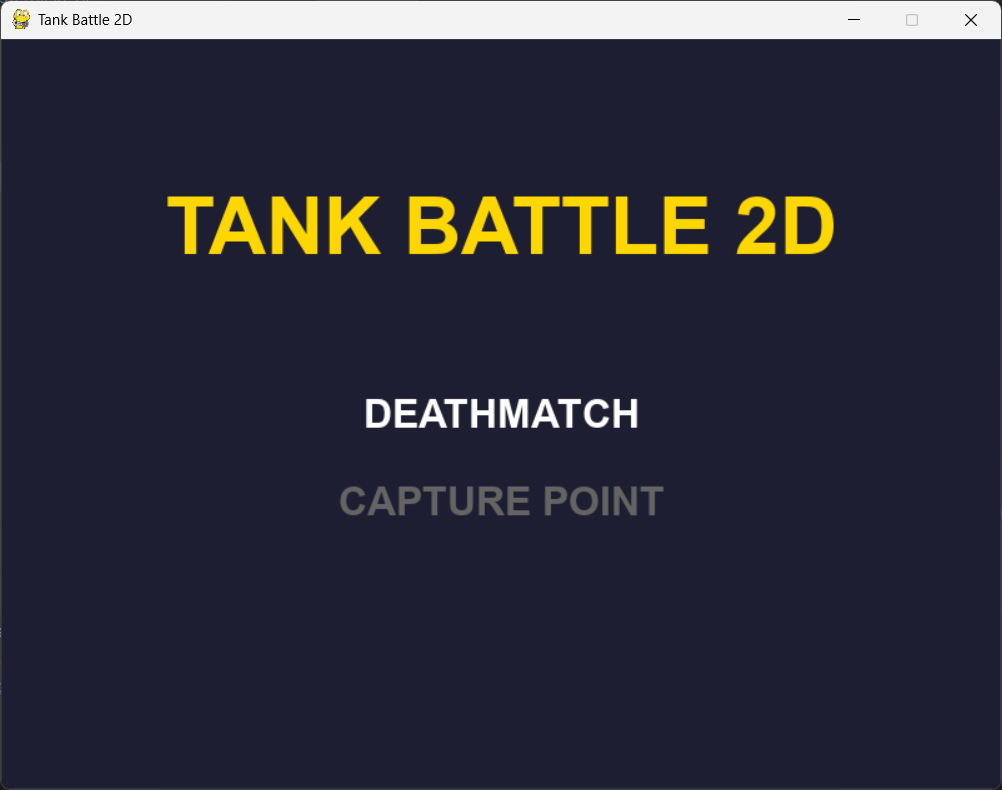
\includegraphics[width=\linewidth]{figures/Strona_glowna.png}
    \caption{Menu główne}
\end{figure}
 
\section{Ekran rozgrywki - tryb Deathmatch}
 
Ekran rozgrywki wtrybie Deathmatch zawiera:

\begin{itemize}
    \item Arenę 800x600 pikseli zlosowo wybraną mapą zfolderu Maps/
    \item Czołg gracza (kolor zielony, sterowanie strzałkami + spacja dostrzału)
    \item Od 1 do 3 czołgów przeciwnika sterowanych przez AI Minimax
    \item Pasek zdrowia nad każdym czołgiem (2 punkty zdrowia maks.)
    \item Ikony aktywnych power-upów
    \item Pojawiające się losowo power-upy (co 2,5 sekundy próba spawnu)
\end{itemize}

\begin{figure}[H]
    \centering
    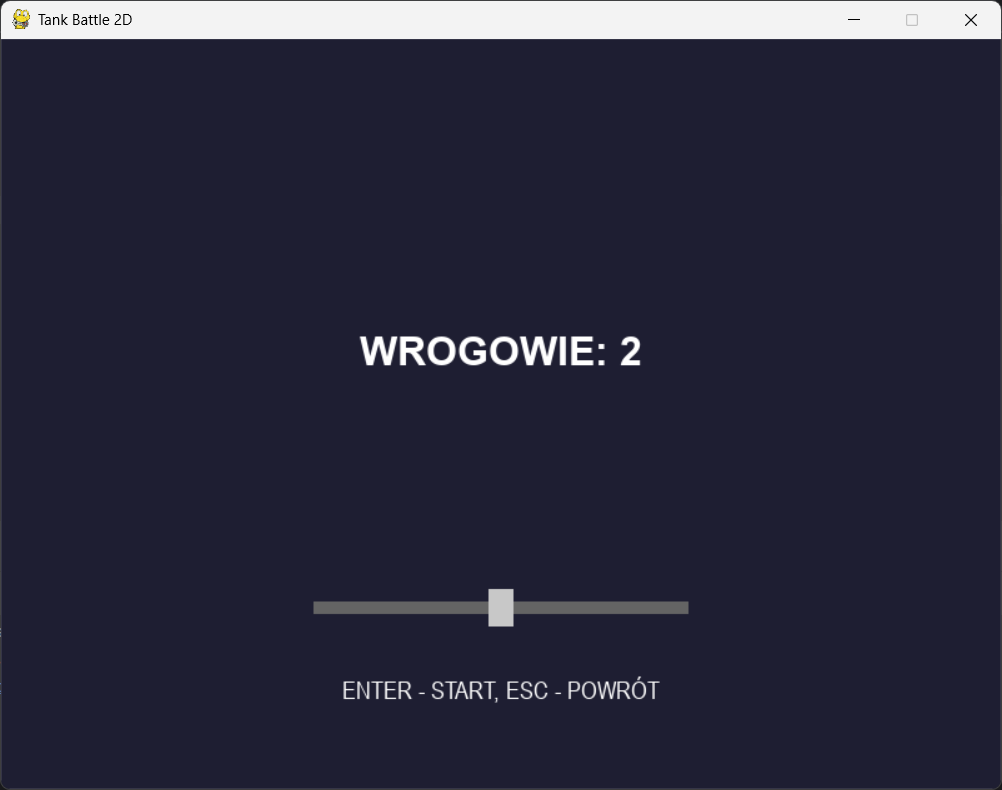
\includegraphics[width=\linewidth]{figures/D_Wejscie.png}
    \caption{Widok wyboru liczebności przeciwników zakres 1-3 (tryb Deathmatch)}
\end{figure}

\begin{figure}[H]
    \centering
    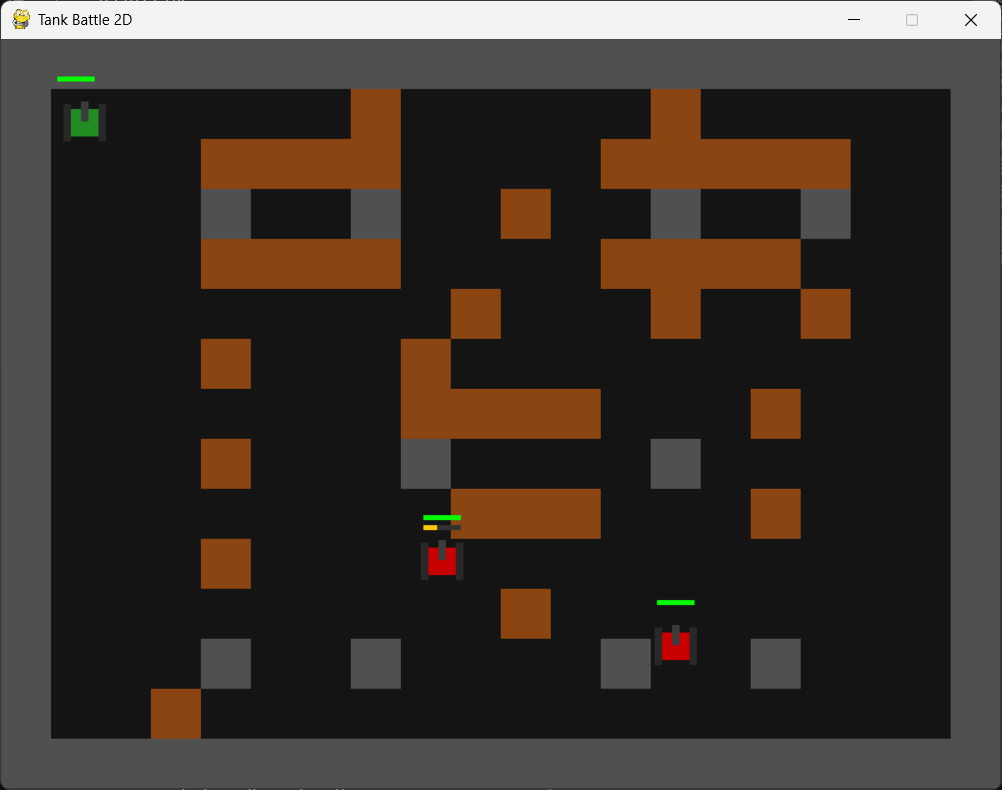
\includegraphics[width=\linewidth]{figures/D.png}
    \caption{Widok rozgrywki w trybie Deathmatch}
\end{figure}
 
Celem gracza jest wyeliminowanie wszystkich przeciwników. Możliwe wyniki rundy:

\begin{itemize}
    \item \emph{Wygrana} - gracz pokonał wszystkich przeciwników
    \item \emph{Przegrana} - gracz został zniszczony
    \item \emph{Remis} - gracz iostatni przeciwnik zostają zniszczeni jednocześnie
\end{itemize}
 
\section{Ekran rozgrywki - tryb Capture Point}
 
W trybie Capture Point arena jest podzielona na siatkę 3x3 sektorów (9 sektorów). 
Na mapie wyświetlana jest strefa przejmowania (na starcie w sektorze centralnym), oraz pasek postępu 
przejmowania u góry ekranu.
 
\begin{figure}[H]
    \centering
    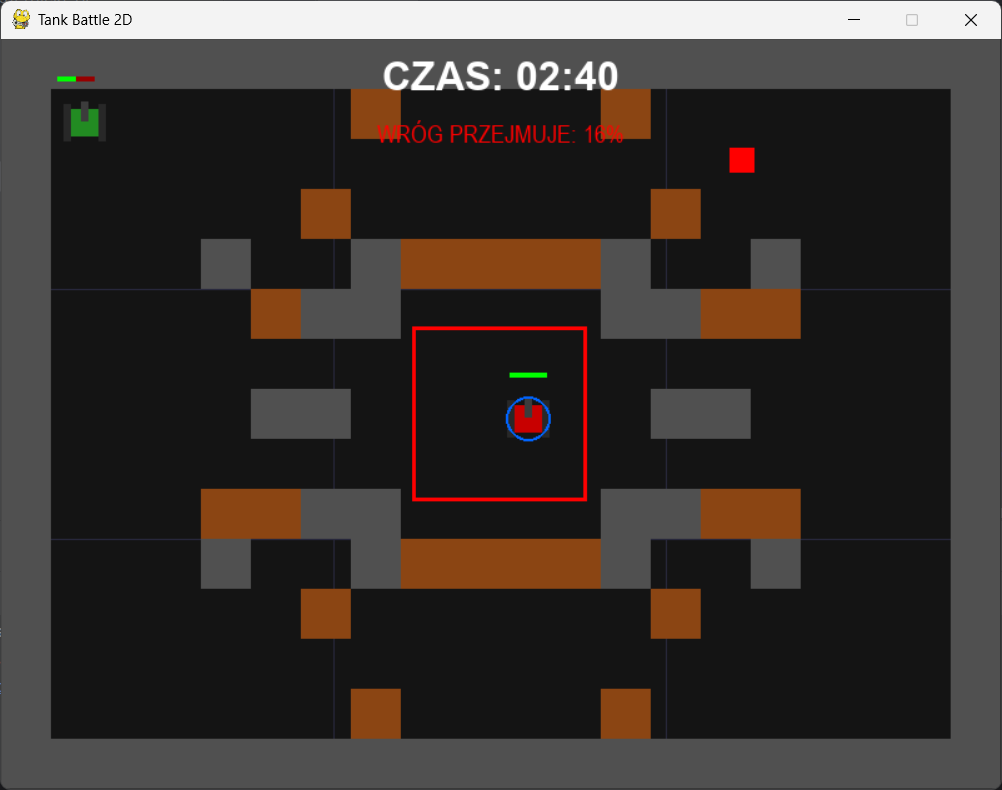
\includegraphics[width=\linewidth]{figures/CP.png}
    \caption{Widok rozgrywki w trybie Capture Point}
\end{figure}

Zasady przejmowania:

\begin{itemize}
    \item Przebywanie gracza w strefie bez przeciwnika zwiększa postęp przejęcia
    \item Przebywanie przeciwnika w strefie bez gracza zmniejsza postęp
    \item Gdy obaj są w strefie, postęp się nie zmienia
\end{itemize}
 
Dynamika rozgrywki:

\begin{itemize}
    \item Co 25 \% przejęcia punkt przenosi się losowo do innego sektora, a po przeciwnej stronie mapy pojawia się nowy przeciwnik
    \item Co 15 \% postępu gracza pojawia się dodatkowy przeciwnik
    \item Aby wygrać należy przejąć punkt do 100\%. Jeśli wróg przejmie punkt do -100\% - gracz przegrywa
    \item Rozgrywka trwa 2 minuty 50 sekund - jeśli w tym czasie nikt nie osiągnie 100\%, runda kończy się jako ,,koniec czasu''
\end{itemize}
 
\section{System power-upów}
 
Power upy tobonusy pojawiające się losowo na mapie wwolnych miejscach (poza ścianami). Każdy power-up 
znika automatycznie po 15 sekundach, jeśli nikt gonie zbierze. Na mapie mogą jednocześnie występować maksymalnie 2 power-upy.
 
\textbf{Zielony - Życie} (\texttt{life}):
\begin{itemize}
    \item Dla gracza w Deathmatch: ustawia licznik dodatkowych żyć na 1, gracz wskrzeszany jest po śmierci ze zdrowiem 2/2 
    w pozycji startowej
    \item Dla gracza w Capture Point: zwiększa licznik dodatkowych żyć o 1 i leczy gracza dopełnego HP
    \item Dla wroga (oba tryby): jeśli wróg jest ranny - leczy go do pełnego HP
\end{itemize}
 
\textbf{Niebieski - Pancerz} 

Pochłania jedno trafienie pociskiem albo jedną kolizję z innym czołgiem, poczym znika. 
Efekt graficzny: niebieskie obramowanie wokół czołgu.
 
\textbf{Czerwony - Silny strzał} 

Następny wystrzelony pocisk zadaje 2 obrażenia zamiast 1, co wystarczy do zniszczenia dowolnego czołgu 
jednym strzałem. Efekt znika natychmiast po oddaniu strzału. Efekt graficzny: 
czerwone obramowanie wokół czołgu i czerwono-pomarańczowy kolor pocisku.
 
\section{Przykładowe scenariusze rozgrywki}
 
W ramach demonstracji zachowania AI zarejestrowano 
2 scenariusze rozgrywki, dostępne jako materiał wideo na platformie YouTube.
Pierwszy przedstawia grę (zachowanie przeciwników) w trybie Deathmatch, drugi
przedstawia grę (zachowanie przeciwników) w trybie Capture Point.

\vspace{10pt}
\textbf{Rozgrywki w trybie Deathmatch:}

\textit{Film :} \href{https://www.youtube.com/watch?v=3lvFnlsOaLk}{https://www.youtube.com/watch?v=3lvFnlsOaLk}
 
\vspace{5pt}
\textbf{Rozgrywka w trybie Capture point:}

\textit{Film:} \href{https://www.youtube.com/watch?v=EoK7oQob9l0}{https://www.youtube.com/watch?v=EoK7oQob9l0}
 
\section{Instrukcja uruchomienia aplikacji}

\begin{enumerate}
    \item Uruchomić środowisko PyCharm.
    \item Sklonować repozytorium projektu z~serwisu GitHub poleceniem: git clone \url{https://github.com/lukaszwarzocha/Projekt_SI.git}
    \item Pobrać bibliotekę pygame poleceniem pip install pygame w terminalu wbudowanym w PyCharm 
    lub przez interfejs zarządzania pakietami.
    \item Uruchomić plik main.py (prawym przyciskiem myszy na pliku potem Run 'main', lub skrótem Shift+F10).
\end{enumerate}

